\documentclass{beamer}
\usepackage[utf8x]{inputenc}
\usepackage{graphicx}
\usepackage{tikz}    
\graphicspath{{./R/}}

\usepackage[outputdir=latex.out]{minted}
\usepackage[T1]{fontenc}


\usetheme{TUM}

\title[Example Presentation]{Long Version of the Example Presentation Title}

\author[Short Name]{Your Full Name}
\institute{Technische Universität München}

\date{Presentation Date}

% Customize alert
\setbeamercolor{alerted text}{fg=TUMZusatzfarbeBlau3}
\setbeamerfont{alerted text}{series=\bfseries}

\begin{document}
\maketitle

\begin{frame}{Lists}
\begin{itemize}
	\item Sample List Item
	\item Sample List Item
	\begin{itemize}
		\item Sample List Subitem
		\item Sample List Subitem
	\end{itemize}
	
	\item[$\Rightarrow$] Other Label List Item
\end{itemize}
\end{frame}

\begin{frame}{Tables}
\centering
\begin{table}
\begin{tabular}{@{::}l|c|c|r@{::}}
	\hline 
	left & center & center & right \\ 
	\hline 
	aligned & \multicolumn{2}{c|}{aligned} & aligned \\ 
	\hline 
	column & column & column & column \\ 
	\hline 
\end{tabular}

\label{tab1}
\caption{Caption text for table} 
\end{table}
\end{frame}

\begin{frame}[fragile=singleslide]{Listing}
\begin{minted}{cpp}
#include <iostream>

int main() {
  std::cout << "hello, world" << std::endl;
  return 0;
}
\end{minted}
\end{frame}

\begin{frame}{Figures}
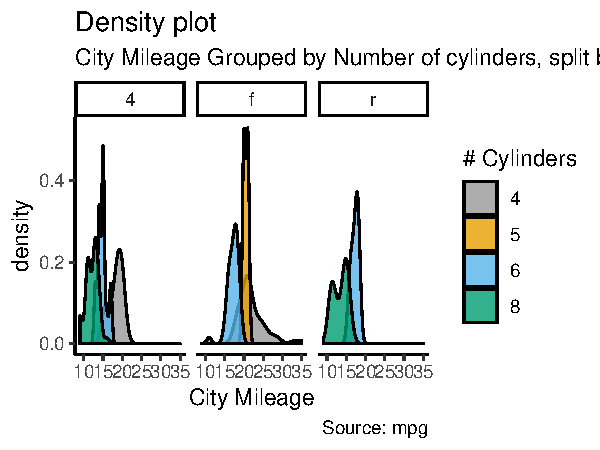
\includegraphics{example.pdf}
\end{frame}

\begin{frame}{Animation}
\only<1>{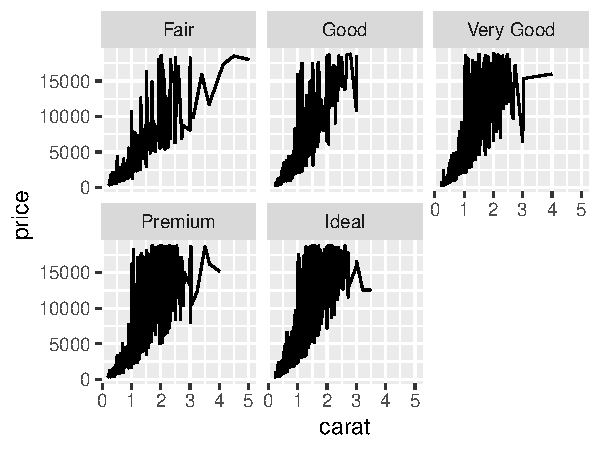
\includegraphics{animation_1.pdf}}

\only<2>{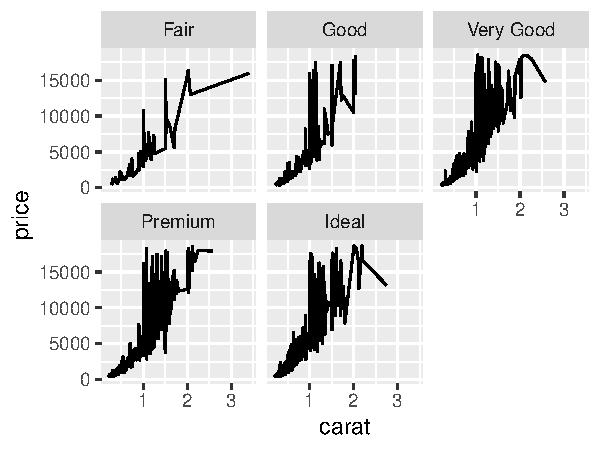
\includegraphics{animation_2.pdf}}

\only<3>{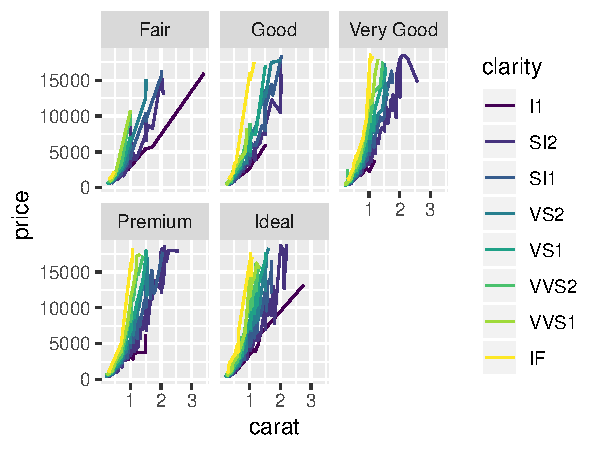
\includegraphics{animation_3.pdf}}

\only<4>{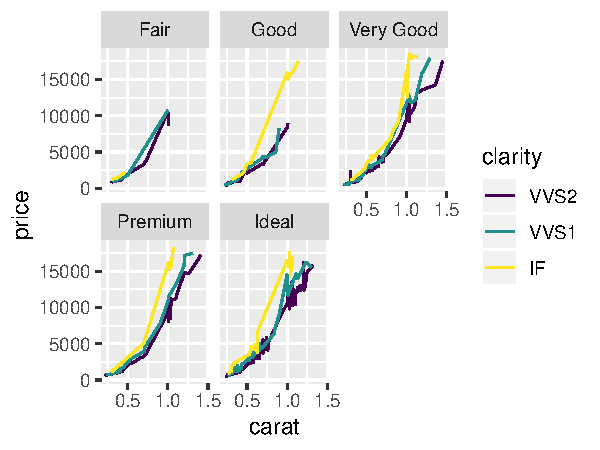
\includegraphics{animation_4.pdf}}
\end{frame}


\end{document}
